\documentclass{article}
\usepackage{chemstyle,mciteplus,notes2bib,rsc,siunitx,url}
\usepackage[version=3]{mhchem}

%%%%%%%%%%%%%%%%%%%%%%%%%%%%%%%%%%%%%%%%%%%%%%%%%%%%%%%%%%%%%%%%%%%%%
% Some (very simple) new commands are defined.
%%%%%%%%%%%%%%%%%%%%%%%%%%%%%%%%%%%%%%%%%%%%%%%%%%%%%%%%%%%%%%%%%%%%%
\providecommand*\acro[1]{\textsc{#1}}
\providecommand*\BibTeX{\acro{Bib}\kern-.08em\relax\TeX}
\providecommand*\cs[1]{\texttt{\char`\\#1}}
\providecommand*\CTAN{\textsc{CTAN}}
\providecommand*\file[1]{\texttt{#1}}
\providecommand*\pkg[1]{\textsf{#1}}

%%%%%%%%%%%%%%%%%%%%%%%%%%%%%%%%%%%%%%%%%%%%%%%%%%%%%%%%%%%%%%%%%%%%%
% Meta-data for this paper
%%%%%%%%%%%%%%%%%%%%%%%%%%%%%%%%%%%%%%%%%%%%%%%%%%%%%%%%%%%%%%%%%%%%%
\title{\LaTeX\ for chemists: filling in the gaps}
\author{Joseph Wright}

\begin{document}
\maketitle

\begin{abstract}
\LaTeX\ is traditionally strongly favoured by mathematicians
and physicists.  Use by chemists has tended to remain on the
`physical' side of the subject.  Support for the particular
needs of chemists has therefore be somewhat variable.  I have
been involved with a selection of new or improved packages,
which seek to address some of the gaps.
\end{abstract}

\section{Introduction}

\LaTeX\ has a whole range of packages available, aimed at
almost the entire range of (academic) pursuits.  However, gaps
still arise, and are filled by interested users.  For chemists,
despite the existence of some very useful tools, gaps have
remained.  As I have worked with \LaTeX, I have worked to fill
some of those gaps, as far as I have been able.  This article
gives an overview of the areas I have contributed to, as well
as highlights from others, and showing some gaps that remain.
All of my packages are available from \CTAN\ in the usual
manner: to keep the bibliography a little shorter, these are
not formally cited although other people's packages are.

Some chemistry-focussed packages will be mentioned in the rest
of this article.  However, one which deserves particular
mention here is \pkg{mhchem} \cite{Hensel2007}.  This allows
very simple input of chemical formulae (and simple in-line
equations). Thus, it allows you to write \verb|\ce{H2SO4}| to
get \ce{H2SO4}, \verb|\ce{CH2=CH-C#CH}| to get
\ce{CH2=CH-C#CH}, or
\begin{verbatim}
\ce{2H2 + O2 -> 2H2O}
\end{verbatim}
and get
\begin{equation}
  \ce{2H2 + O2 -> 2H2O}.
\end{equation} 
It is a tool no chemist using \LaTeX\ should be without.

\section{Bibliography tools}

\subsection{\BibTeX\ styles}

One area where chemists seem to have unusual requirements is in
creating bibliographies.  To begin with, as a chemist the name
is wrong: it is the \emph{References} section.  The most basic
requirement for everyone using \BibTeX\ is appropriate style
files.  When I started using \LaTeX, I found the
\file{pccp.bst} \BibTeX\ style, based on the journal
\emph{Physical Chemistry Chemical Physics}.  However, there
were problems with the output.  I therefore wrote my own style,
\file{rsc.bst}, based on the general requirements of the Royal
Society of Chemistry (\acro{RSC}); as a U.K.-based worker, the
\acro{RSC} style is one I follow for my own documents.  Over
time, \file{rsc.bst} was joined by \file{angew.bst}, aiming at
the requirements of \emph{Angewandte Chemie} (arguably the
`top' general chemistry journal: I'm sure a lot of American
chemists would disagree!). These files, plus some utility
macros, ended up in a package called \pkg{rsc}. Later, the
utility macros moved elsewhere, but the \pkg{rsc} survives in
modified form.

The \pkg{achemso} package was originally written by Mats
Dahlgren, and provided a \BibTeX\ style following the
requirements of the American Chemical Society (\acro{ACS}).
Once I started using the style, I spotted some issues.
Contacting the author, I found he no longer had time for
package maintenance.  So, as much by accident as by design, I
took over \pkg{achemso}.  A complete re-write resulted, with
improvement to the \BibTeX\ style and the accompanying \LaTeX\
package. More recently, I've re-written the package again so that
it fits in with the submission system at the \acro{ACS}: this
hopefully makes submitting articles a bit easier. 

\subsection{Bibliography packages}

Beyond \BibTeX\ styles, chemists have two important
requirements for bibliographies.  First, the idea of
`compound' references is common.  Most chemistry journals use
numerical citations, rather than the author--date system.
It is very common to want a single reference number to refer to
several related journal articles.  The \pkg{mcite} package
\cite{Ohl2005} can do this, but with very limited control of
the results. In particular, it s common in chemistry to give
each reference a letter inside a long list, such as
\begin{quote}
  [4] (\emph{a}) G.~Alberti, M.~Casciola, U.~Costantino,
  A.~Peraio and E.~Montoneri, \emph{Solid State Ionics}, 1992,
  \textbf{50}, 315--322; (\emph{b}) G.~Alberti, M.~Casciola,
  U.~Costantino and R.~Vivani, \ldots
\end{quote}
The \pkg{mcite} package cannot do this automatically.  So I
began to consider the issue, and to ask on
\texttt{comp.text.tex} if anyone had contact details for the
author of \pkg{mcite}. Luckily, Michael Shell was interested in
the other extensions to \pkg{mcite}: the result was the
\pkg{mciteplus} package \cite{Shell2008}, which \emph{can}
generate the desired output with control of formatting.
Although I did not write any of \pkg{mciteplus}, the aim of
making sub-lists inside each reference is included there
specifically because I worked with him to get it working. Thus
the example citation above can be given in the source simply as
\begin{verbatim}
\cite{Alberti1992,*Alberti1996}
\end{verbatim}
which results in nicely-formatted output
\cite{Alberti1992,*Alberti1996}.  This document uses my
\file{rsc.bst} \BibTeX\ style, which sets up \pkg{mciteplus}
to follow the requirements of the \acro{RSC}; for example, this
instructs \pkg{mciteplus} to use a sub-list, and to make the
sub-labels italic.

The second thing that chemists like to do is mix notes and
references.  This can be done by creating a \BibTeX\ database
of notes for every document you write to contain the
information, but it is tedious.  A much better idea would be to
add the text directly into the body of the file, and have it
move automatically to the bibliography section.  To achieve
this, I wrote the \pkg{notes2bib} package.  The package works
by creating a database for the notes during the \LaTeX\ run,
and then ensuring it is added to the list of files to be
processed by \BibTeX. This means it is `neutral' with respect
to sorting of bibliographies and packages used, such as
\pkg{cite} \cite{Arseneau2009}, \pkg{natbib} \cite{Daly2009},
\pkg{biblatex} \cite{Lehman2009}, \etc.  Using \pkg{notes2bib}
implies using numerical citations: the citations do not make
much sense with the author--year system!  Using the package
requires only inclusion of one or more \cs{bibnote}s in the
source, although it is possible to convert \cs{footnote} or
\cs{endnote} entries into \cs{bibnote} data automatically.  For
example, you could write
\begin{verbatim}
\bibnote{An example bibliographic note}
\end{verbatim}
and this would give \bibnote{An example bibliographic note}.

\section{Utilities}

The \pkg{mhchem} package is probably the most useful general
utility package for chemists.  However, this leaves a few gaps
that can happily be filled.  Initially, I provided a package
with the \pkg{rsc} bundle to do this.  However, later it became
clear there was a better approach.  The \pkg{chemstyle} package
inherited the utilities from \pkg{rsc}, along with new
functions.  For example, this gives the macros \verb|\tBu|,
\verb|\iPr|, \etc. to give alkyl radicals: \tBu, \iPr, \etc. It
also provides items such as the `standard state' symbol, to
allow you to produce $\Delta H^{\standardstate}$ easily.

The main aim of \pkg{chemstyle} is to help maintain
consistency.  By specifying the journal style to follow, the
package allows float captions, cross-referencing and so on to
follow the choices of the publication given.  This is a lot
easier than trying to remember the choices of every separate
journal. It also loads a number of useful packages for the
chemist, including my own \pkg{chemscheme}.

\section{Graphics: the `scheme'}

The concept of a `scheme' is one that non-chemists find
difficult to understand: they expect the name `equation' to
be used.  An equation to most synthetic chemists is a simple,
broadly non-graphical item, such as Equation~\ref{eqn}.
\begin{equation}
  \ce{2H2 + O2 -> 2H2O} \label{eqn}
\end{equation}
In contrast, a scheme is a more complex, graphically-rich item,
such as \ref{sch}. The example here is simple by the standards
of many schemes in the research literature.  Several packages
are available for generating the graphics directly in \LaTeX.
However, producing anything beyond the most simple scheme
becomes very difficult using text-based tools.  I, like almost
every synthetic chemist, use the commercial package
\textsc{ChemDraw}\bibnote{See
\url{http://www.cambridgesoft.com}} to produce my schemes.
\begin{scheme}
  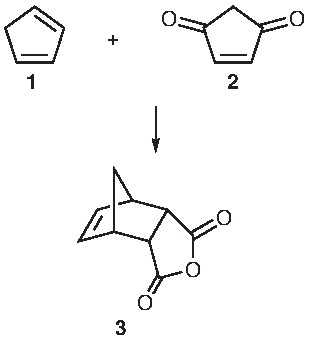
\includegraphics{Scheme}
  \caption{A simple scheme}
  \label{sch}
\end{scheme}

Rather than trying to provide a package to tackle directly
producing schemes in \LaTeX, the \pkg{chemscheme} package aims
to solve two lesser problems.  The first aim of
\pkg{chemscheme} is to provide an `out of the box' float for
schemes.  Chemists expect the scheme to be near `here' if
possible, so this is the case with the \texttt{scheme} float.
Thus the example scheme used here is produced using
\begin{verbatim}
\begin{scheme}
  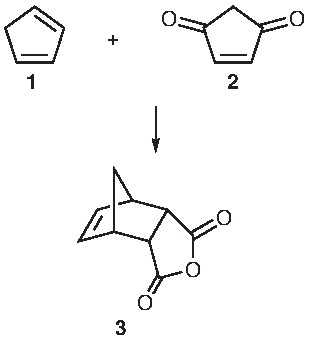
\includegraphics{Scheme}
  \caption{A simple scheme}
  \label{sch}
\end{scheme}
\end{verbatim}

The second aim is more complex.  The use of reference numbers
for chemicals in graphics is very common.  Two packages exist
to automate this in the text: \pkg{bpchem} \cite{Pedersen2004}
and \pkg{chemcompounds} \cite{Schenk2006}.  However, neither
can work with graphical content.  Using \pkg{PSfrag}
\cite{Carlisle1998}, the \pkg{chemscheme} package makes
automatic substitution easy for \file{.eps} graphics. This is
achieved by the \cs{schemeref} macro, which works with a
temporary marker in the input.  By using \pkg{pst-pdf}
\cite{Gasslein2008} this can also be used with PDF\LaTeX.

\section{\pkg{biblatex} bibliographies}

The \pkg{biblatex}, currently available with beta status, is a 
completely new way to produce bibliographies from a database. 
The current version uses \BibTeX, but does not need dedicated
style files to do this. Instead, it requires \LaTeX\ files containing
formatting instructions.  I've written some of these for chemists
and other scientists: \pkg{biblatex-chem} to cover the same journals
as \pkg{rsc} and \pkg{achemso}, \pkg{biblatex-nature} for 
\emph{Nature}-like formatting and \pkg{biblatex-science} to emulate
the journal \emph{Science}.

\section{Further afield}

Beyond the focus on chemistry, one package in particular
deserves mention here.  Using units with numbers is common
across the whole of science.  The \pkg{siunitx} package
provides a wide range of tools for typing units and values. For
example, the input
\begin{verbatim}
$R = \SI[dp=3]{8.314472}
  {\joule\per\mole\per\kelvin}$
\end{verbatim}
gives the typeset result $R = \SI [dp=3] {8.314472}
{\joule\per\mole\per\kelvin}$, while
\begin{verbatim}
$R = \SI[dp=5,per=slash]{8.314472}
  {\joule\per\mole\per\kelvin}$
\end{verbatim}
gives $R = \SI [dp=5,per=slash] {8.314472}
{\joule\per\mole\per\kelvin}$.  This type of format control is
available either on a per-macro basis or by setting package
settings in the document.  The aim of \pkg{siunitx} is
therefore to allow units and values to have a single input
syntax but give a range of output formats: this makes working
with different publishing requirements much easier.

\bibliographystyle{rsc}
\bibliography{ChemTeX}

\end{document}
